A study of the influence of the fiber diameter in the tritium measurement was carried out. For this task, simulations of a single $20~\cm$ length scintillating fiber and two different diameters, $1~\mm$ and $2~\mm$ (the commercial options given for Saint-Gobain), were compared. An important point is how the fiber diameter affects the cosmic ray detection, which is an important component of the TRITIUM monitor background. The energy deposited in the scintillating fiber by a cosmic ray is proportional to the active volume crossed, which is larger for $2~\mm$ fibers. Therefore, the cosmic ray signal would be larger for $2~\mm$ diameter fibers. The objective of this study is to find which minimizes the background in the energy region of tritium detection, up to $18~\keV$ (region of interest, ROI). For this study, the tritiated water source was replaced by a cosmic ray source, generated by the CRY library\footnote{CRY library, Cosmic-Ray Shower library} \cite{CRYwebsite, CRYpaper}. The CRY library is a package based on object-oriented technology and implemented in the C++ programming language. This library generates cosmic-ray shower distributions for different particles (muons, neutrons, protons, electrons, photons and pions). The cosmic source shape used in this simulation is a horizontal square of $1 \times 1~\meter ^2$ located at a height of $35~\cm$ (above the detector) with the typical distribution of cosmic particles at sea level. The distribution of energy deposited in scintillating fibers for $1~\mm$ and $2~\mm$ diameters by cosmic rays is shown in Figure \ref{fig:DiameterComparison}. As can be seen in the figure, a smaller background is measured for fiber diameters of $1~\mm$, which allow to achieve a lower minimum detectable activity MDA of the detector. There are other reasons that may favor the use of $2~\mm$ fibers, such as their greater rigidity and better flow of water through them. Thus, a complementary experimental study is needed to assess the most appropriate diameter size for the scintillating fibers.

\begin{figure}[hbtp]
\centering
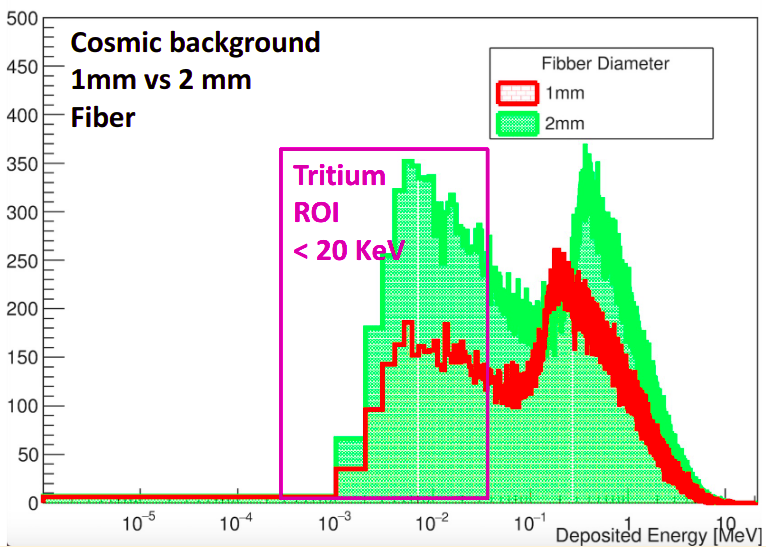
\includegraphics[scale=0.4]{Figures/8SimulationsResults/81TRITIUMDesign/814Diameter/ComparisonDiameter.png}
\caption{Comparison of the energy deposition by cosmic rays in scintillating fibers of $1~\mm$ and $2~\mm$ diameter.\label{fig:DiameterComparison}}
\end{figure}o